\documentclass[a4paper, 11pt]{article}

\usepackage[utf8]{inputenc}

\usepackage[T1]{fontenc}

\usepackage[english]{babel}

\usepackage{graphicx}

\usepackage{multicol}

\usepackage{floatrow}

\usepackage[margin = 1in]{geometry}

\usepackage{float}

\usepackage[hidelinks, urlcolor=cyan]{hyperref}

\usepackage{url}

\usepackage{natbib}

\bibliographystyle{abbrvnat}
\setcitestyle{authoryear,open={(},close={)}}

\usepackage{csquotes}

\usepackage{fancyhdr}

%\addbibresource{references.bib}

\title{\Large BINF-402 Project \\
\huge Differential expression analysis of micro-RNA transcriptome between pancreas, prostate and gastrocnemius medialis tissues}


\author{Léopold Guyot}

\date{\today}

\begin{document}

\pagestyle{fancy}
\setlength{\headheight}{32.3pt}
\fancyhead{}\fancyfoot{}
\fancyhead[L]{
\includegraphics[width = 0.2\textwidth]{Figures/LOGO_Universite _libre_bruxelles.png}}
\fancyhead[R]{Differencial expression analysis of microRNA transcriptomes}
\fancyfoot[R]{\thepage}

\maketitle

\begin{multicols}{2}
\section{Introduction}
This analysis investigates microRNA expression variations across three distinct tissues; prostate gland, pancreas body, and gastrocnemius medialis. For this a simple workflow will be used, consisting of quality control of the reads, followed by a filtering, then a mapping to finish we a classic differential expression analysis. The goal is to unveil tissue-specific expression patterns of miRNA. Tissue selection is strategic, anticipating closer miRNA expression patterns between prostate and pancreas, both glandular, and unique signatures in gastrocnemius medialis, a muscle tissue.

\section{Methods}
All the data processing was done using the language R \citep{Rlang} and several packages. All graphs have been realize with the ggplot2 package \citep{ggplot2} and basic data manipulations have been done with the help of the tidyr package \citep{tidyr}. Note that for each section, the relevant scripts are indicated. Each script name is clickable to acces code through the associated github link. The link to the github repo is
{\scriptsize \href{https://github.com/leopoldguyot/BINF-402_Transcriptomic_Project/}{https://github.com/leopoldguyot/BINF-402\_Transcriptomic\_Project/}}
\subsection{Data Retrieval}
\begin{scriptsize}
	\textbf{Script associated : \href{https://github.com/leopoldguyot/BINF-402_Transcriptomic_Project/blob/main/retrieve_data.R}{retrieve\_data.R}}
\end{scriptsize}



All the data sets used in this project have been retrieve from the ENCODE database \citep{luo2020new}.
Three tissues have been selectionned; pancreas body, prostate gland and the gastrocnemius medialis tissue.
For each tissue, data used was coming from two distinct experiments, each comprising two replicates, thereby totaling four replicates per tissue (cf. \href{https://github.com/leopoldguyot/BINF-402_Transcriptomic_Project/blob/data/sample_table_links.csv}{"data/sample\_table\_links.csv"} for file accession numbers).

The original UCSC hg38 genome was used as reference for the mapping. The NCBI accession for this genome is \href{https://www.ncbi.nlm.nih.gov/datasets/genome/GCF_000001405.26/}{GCA\_000001405.26}.


\subsection{Read Quality Control}
\begin{scriptsize}
	 \textbf{Scripts associated : \href{https://github.com/leopoldguyot/BINF-402_Transcriptomic_Project/blob/main/reads_mapping.R}{reads\_mapping.R},\\
	 	  \href{https://github.com/leopoldguyot/BINF-402_Transcriptomic_Project/blob/main/Quality_control_stats.R}{Quality\_control\_stats.R}, \\
	 	  \href{https://github.com/leopoldguyot/BINF-402_Transcriptomic_Project/blob/main/quality_control.R}{quality\_control.R}}
\end{scriptsize}


A preliminary analysis done using the Rqc package \citep{Rqc} revealed notable issues with the quality of the sequencing reads. Others statistics have been retrieve and used to find the problems and adapt the processing of the reads. 

Red line in the summary Figure \ref{fig:cycles_mean} depict the evolution of the quality trough the cycles for the unprocessed reads, indicate a substantial low mean quality for the initial 5 cycles (certainly due to a adapter) and a significant decrease from the 43rd cycle to the end of the reads (mean quality of the cycles of unprocessed reads is highlighted by the red line in the figure).

To address these quality issues, an initial processing step was implemented using the QuasR package \citep{QuasR} (for performance reasons). This step involved trimming the first 5 and the last 7 cycles of the reads (additionally, reads with unidentified residues were filtered out). The result is visible with the green line in Figure \ref{fig:cycles_mean}. Even after this first step, a persistent decrease in mean quality throughout the remaining cycles was still observed.

In response to the persistent decline in mean quality, a second processing step was undertaken. In this step, reads were filtered to retain only those with a mean quality higher than 20. The outcome of this filtering is illustrated by the blue line in Figure \ref{fig:cycles_mean}. This additional processing step led to a global increase in mean quality across the entire read length and a stable read quality through cycles, the previous trend of decreasing quality has been effectively mitigated.


\begin{figure}[H]
    \centering
    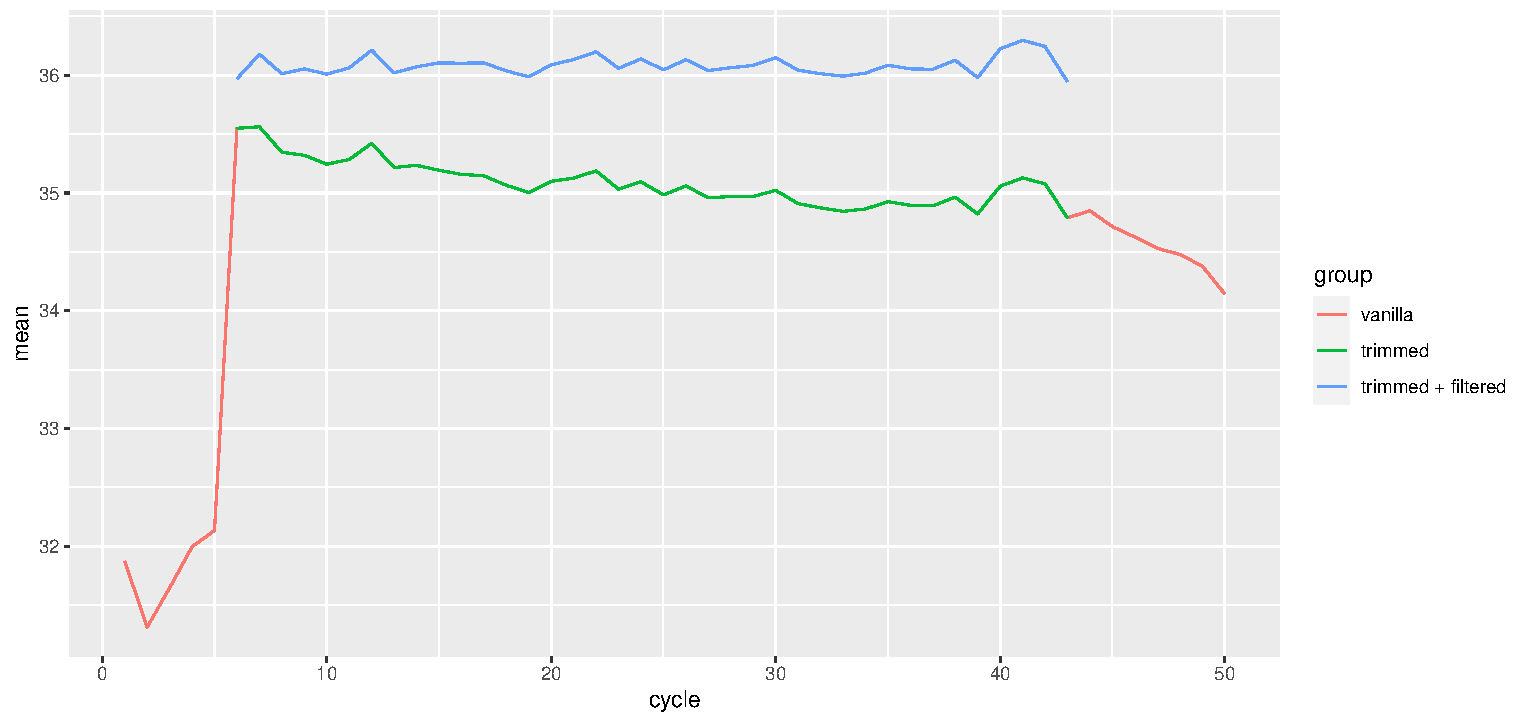
\includegraphics[width=1\columnwidth]{Figures/QC_plots/mean_per_group_and_cycles.pdf}
    \caption{\footnotesize{ Graph of the mean quality (Phred score) for each cycle. Each line is composed of the mean quality values of all the reads contained on the 12 datasets (4 replicates and 3 tissues). The red line is for the unprocessed data, the green line for the data with trimmed reads and the blue line for the data with trimming and filtering.}}
    \label{fig:cycles_mean}
\end{figure}

In the following section, the mapping performance for each version of the data (unprocessed, with trimming, with trimming and filtering) will be explored. This analysis will provide insights into how the quality enhancements impact the alignment of reads.

\subsection{Mapping}
\begin{scriptsize}
	\textbf{Script associated : \href{https://github.com/leopoldguyot/BINF-402_Transcriptomic_Project/blob/main/reads_mapping.R}{reads\_mapping.R}} 
\end{scriptsize}


Before mapping, an index of the hg38 genome was created. The mapping was conduct on unprocessed data sets, data sets with reads trimming and data sets with trimming and filtering. Both indexing and mapping were carried out with the Rsubread package \citep{Rsubread}.

By comparing the mapping proportions, we can clearly see the impact of quality control on the mapping performance (cf Fig.\ref{fig:mapping}). With no processing on the reads, the proportion is really low with a median value under 10\%, some data sets have mapping proportion that do not go above 2\%. After a first trimming of the start and end of the reads, the improvement is quite visible, as we go from 10\% to slightly under 75\% of median mapping proportion. And the minimal proportion is not going under 65\%. With the extra step of filtering the reads, the median proportion slightly increase and is above 75\%. And the minimal proportion is 68\%. 


\begin{figure}[H]
    \centering
    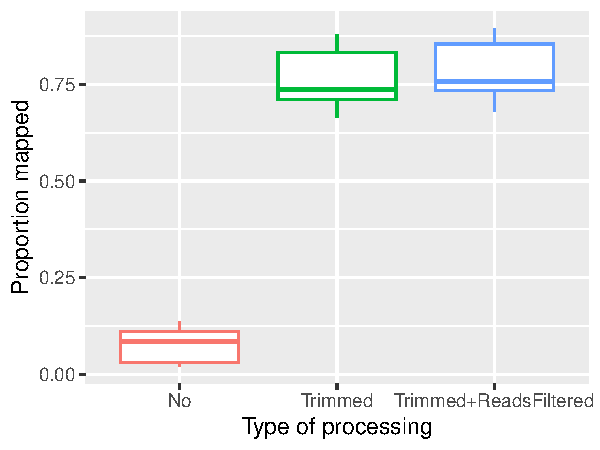
\includegraphics[width=1\columnwidth]{Figures/mapping_props.pdf}
    \caption{\footnotesize{Graph of the proportion of reads mapped based on the read processing method used. For each category, n = 12 (4 replicate for 3 tissues). The first category "No" stands for the case with no processing.}}
    \label{fig:mapping}
\end{figure}


\subsection{Differential Expression Analysis}
\begin{scriptsize}
	\textbf{Script associated : \href{https://github.com/leopoldguyot/BINF-402_Transcriptomic_Project/blob/main/differential_expression_analysis.R}{differential\_expression\_analysis.R}} 
\end{scriptsize}


Before running the proper differential analysis. A feature count was carried out with the Rsubread package \citep{Rsubread}. The annotation used was the one contained within the package. 

The differential expression analysis was done using the DESeq2 package \citep{DESeq2} the workflow employed is inspired from the workflow presented in Chapter 4 of the "Omics Data Analysis" UCLouvain course from Laurent Gatto \citep{Gatto_Loriot}.

The big strength of DESeq2 is that it will correct the count matrix to account for potential bias between data sets. These bias are for instance difference in sequencing depth across sample (quite present in this analysis cf. Fig \ref{fig:depth}) and the difference in library composition that can lead to bad normalisation if not taken into account. To accomplish this normalisation, DESeq2 will compute geometric mean for each gene then it will use these values and create a new matrix that consist of the counts divided by their associated geometric mean. After that it will use this new matrix to build scaling factors for each sample, and finally applying this scaling factor to the original counts.
\begin{figure}[H]
	\centering
	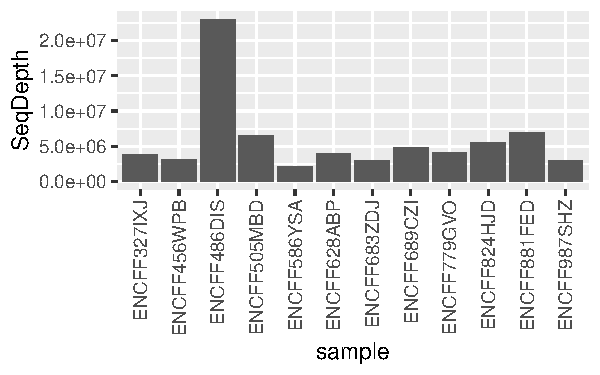
\includegraphics[width=1\columnwidth]{Figures/differential_analysis/depth.pdf}
	\caption{\footnotesize{Graph of the proportion of reads mapped based on the read processing method used. For each category, n = 12 (4 replicate for 3 tissues). The first category "No" stands for the case with no processing.}}
	\label{fig:depth}
\end{figure}

A first exploration of the normalized count matrix was done using dimension reduction method. To avoid that largely expressed features impact strongly the new dimension reduction, at the expense of features with lower expression profile, a regularized-logarithm transformation was carried out. This type of transformation allow low and high expressed features to have same weight during the dimension reduction step. A classic Principal Component Analysis was conduct. Then an unsupervised clustering algorithm (using k-means method) was used to assess if the different tissues types can be identify based on the mi-RNA expression pattern.

To access the differential analysis, DESeq2 employs a step that will estimate the dispersion parameter of the negative-binomial distribution. This estimation rely to the assumption that features of similar expression levels have similar dispersions and will thus use information coming from similar expressed features to estimate the dispersion values. Then it proceeds with extra step that will lead to reduce false positives in the differential expression analysis. These steps include, fitting the dispersion values to then shrink the dispersion values toward the values predicted by the curve. The results of the dispersion estimation is visible on the Figure \ref{fig:dispersion}
\begin{figure}[H]
	\centering
	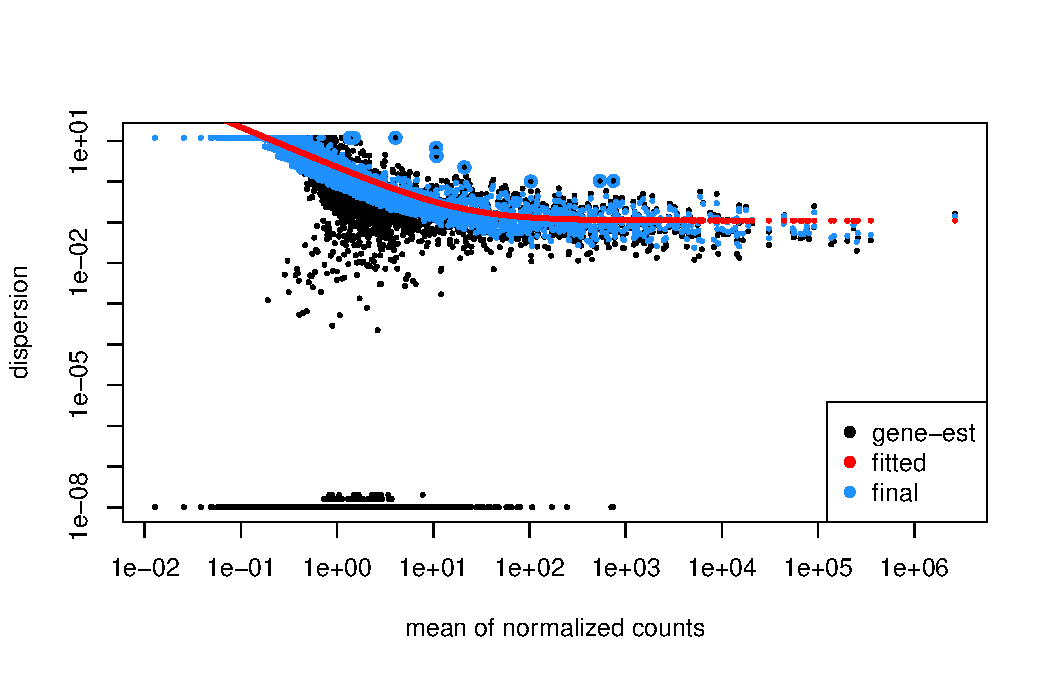
\includegraphics[width=1\columnwidth]{Figures/differential_analysis/dispersion.pdf}
	\caption{\footnotesize{Graph of the proportion of reads mapped based on the read processing method used. For each category, n = 12 (4 replicate for 3 tissues). The first category "No" stands for the case with no processing.}}
	\label{fig:dispersion}
\end{figure}

DESeq2 will then fits a generalized linear model. This model will give us the log2 Fold Change between two sampled type and its associated p-value (the p-value is obtained with Wald test). Due to the high number of statistical tests that need to be carried out, DESeq2 uses Benjamini-Hochberg method to adjust pvalues.To decrease the loss of statistical power associated with the multiple testing correction, DESeq2 filter out the tests that have almost no chance to show a significant fold change. 

The results of this analysis will be explored on the Results section.

%\subsection{Gene Ontology}

\section{Results}

Present the overall results => Differential Expression Analysis


\section{Discussion}
???? maybe not include it
=> things I could Improve


\section{Conclusion}


\bibliography{references}

\end{multicols}
\end{document}
